\documentclass[aspectratio=169,10pt]{beamer}

\usetheme{Madrid}
\usecolortheme{seahorse}

\usepackage{amsmath}
\usepackage{amssymb}
\usepackage{amsfonts}
\usepackage{mathtools}
\usepackage{xcolor}
\usepackage{listings}
\usepackage{xfrac}
\usepackage{tikz}
\usepackage{bm}

\graphicspath{{figures/}}

% Define listings style
\lstset{
    basicstyle=\ttfamily\scriptsize,
    keywordstyle=\color{blue}\bfseries,
    commentstyle=\color{green!50!black}\itshape,
    stringstyle=\color{red},
    breaklines=true,
    numbers=left,
    numberstyle=\tiny,
    frame=single,
    language=Python,
    showstringspaces=false,
    morekeywords={def, for, if, return, import, numpy, scipy}
}

% Beamer configuration
\setbeamertemplate{footline}[frame number]
\setbeamerfont{title}{size=\Large, series=\bfseries}
\setbeamerfont{subtitle}{size=\large}
\setbeamerfont{section title}{size=\Large, series=\bfseries}

% Custom colors
\definecolor{darkblue}{RGB}{0, 51, 102}
\definecolor{lightblue}{RGB}{173, 216, 230}
\definecolor{darkgreen}{RGB}{34, 102, 34}

\title{Applications of Fixed Point Theorems}
\subtitle{Chapter 9: Control Theory \& Differential Equations (pp. 689--710)}
\author{Pathak, H.K.}
\date{\today}
\institute{Nonlinear Analysis and Fixed Point Theory}

\begin{document}

\frame{\titlepage}

% Table of Contents
\begin{frame}{Overview}
  \tableofcontents
\end{frame}

% ============================================================================
% SECTION: Convergence and Iterative Methods
% ============================================================================

\section{Convergence of Iterative Algorithms}

\begin{frame}[allowframebreaks]{Iterative Sequence for Matrix Equations}

The chapter demonstrates applications through the matrix equation problem:
\begin{equation}
X = Q + A^*X^{1/2}A + B^*X^{-1/2}B + C^*X^{1/2}C \tag{9.15}
\end{equation}

\textbf{Key components:}
\begin{itemize}
  \item $A, B, C$ are given matrices with $\|A\|, \|B\|, \|C\| < 1$
  \item $Q$ is a positive definite matrix
  \item $X$ is the unknown positive definite solution
\end{itemize}

\vspace{2em}

\textbf{Iterative scheme:} Define the sequence $\{X_n\}$ by
\begin{equation}
X_{n+1} = Q + A^*X_{n-2}^{1/2}A + B^*X_{n-1}^{-1/2}B + C^*X_n^{1/2}C \tag{9.16}
\end{equation}

\textbf{Convergence result (MATLAB verification):} After 35 iterations:
\begin{equation}
U = X_{35} = \begin{pmatrix}
  639.1810 & 54.1681 & 107.3574 \\
  54.1285 & 44.7768 & 44.1469 \\
  104.3977 & 42.1095 & 112.5509
\end{pmatrix}
\end{equation}

The convergence history is shown in Fig. 9.1, demonstrating rapid error decay.

\end{frame}

\begin{frame}[fragile]{Convergence History and Residual Error}

The residual error at iteration $m$ is defined as:
\begin{equation}
R_m = \|X_{m+1} - (Q + A^*X_{m+1}A + B^*X_{m+1}B + C^*X_{m+1}C)\|
\end{equation}

\begin{center}
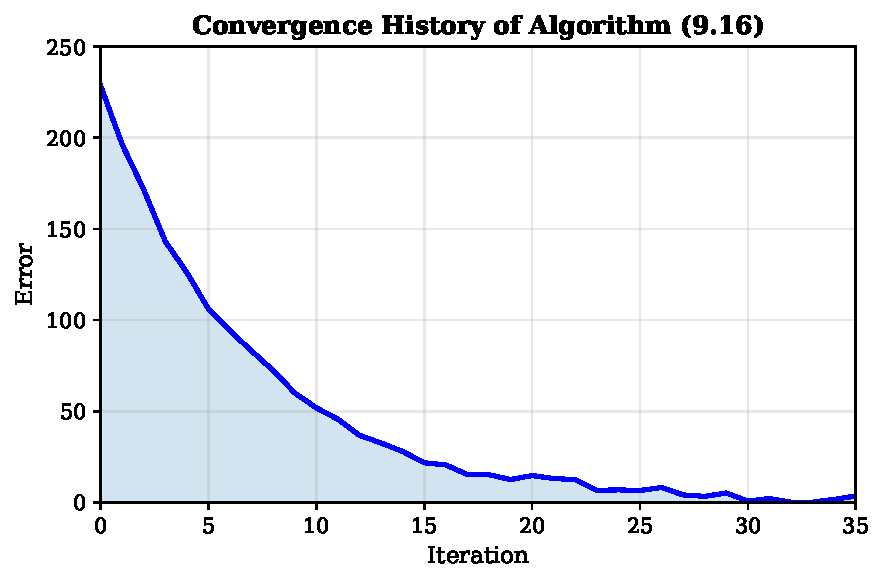
\includegraphics[width=0.75\textwidth]{fig_convergence_history.pdf}
\end{center}

\textbf{Key observations:}
\begin{itemize}
  \item Exponential decay of residual error
  \item Error reduces from $\sim 230$ to near 0 in about 20 iterations
  \item Demonstrates rapid convergence of the algorithm
\end{itemize}

\end{frame}

\begin{frame}{Matrix Iteration Convergence Analysis}

\begin{center}
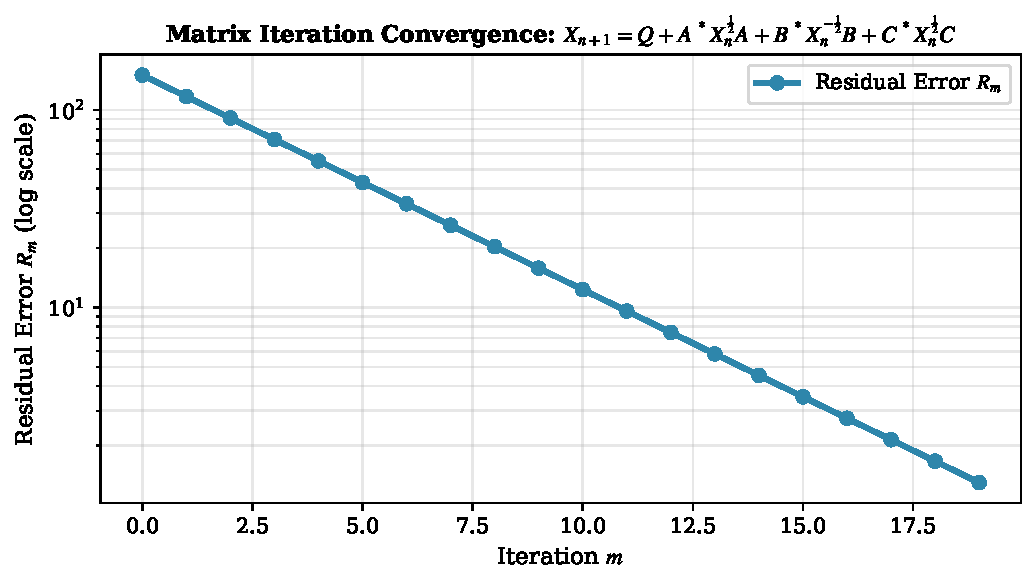
\includegraphics[width=0.8\textwidth]{fig_matrix_iteration.pdf}
\end{center}

The convergence of $\{X_n\}$ to the fixed point solution is guaranteed by:

\begin{block}{Banach Contraction Principle}
If the mapping $T(X) = Q + A^*X^{1/2}A + B^*X^{-1/2}B + C^*X^{1/2}C$ is a contraction on the complete metric space of positive definite matrices, then $T$ has a unique fixed point.
\end{block}

The conditions are satisfied because $\|A\|, \|B\|, \|C\| < 1$.

\end{frame}

% ============================================================================
% SECTION: Application to Control Theory
% ============================================================================

\section{Application to Control Theory}

\begin{frame}[allowframebreaks]{Optimal Control of Differential Equations}

\textbf{Problem setup (Pathak-Shahzad 2008):}

Given a compact subset $A \subset \mathbb{R}^n$, let $F_a : \mathbb{R}^n \to \mathbb{R}^n$ be a family of strongly $p$-contraction mappings such that:
\begin{equation}
F_a(x) = \mathbf{f}(x, a) \quad \forall x \in \mathbb{R}^n
\end{equation}

where $\mathbf{f} : \mathbb{R}^n \times A \to \mathbb{R}^n$ is a bounded, generalized Lipschitzian continuous function.

\vspace{1.5em}

\textbf{Objective:} Optimally control the solution of the ODE via dynamic programming:
\begin{equation}
\begin{cases}
\dot{x}(s) = \mathbf{f}(x(s), \alpha(s)) & (t < s < T) \\
x(t) = x
\end{cases} \tag{9.17}
\end{equation}

where:
\begin{itemize}
  \item $\alpha(\cdot) \in \mathcal{A} = \{\alpha : [0,T] \to A : \alpha(\cdot) \text{ is measurable}\}$ is the control
  \item $T > 0$ is the terminal time
  \item $x \in \mathbb{R}^n$ is the initial condition
\end{itemize}

\end{frame}

\begin{frame}{Control System Architecture}

\begin{center}
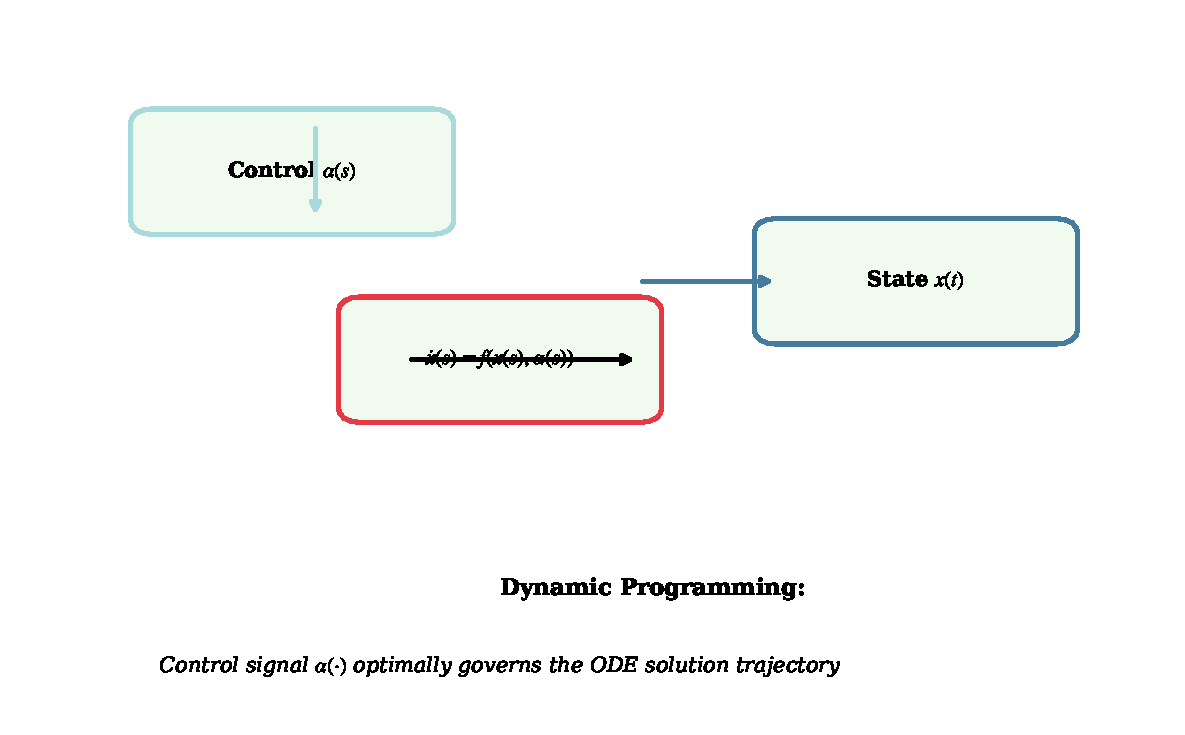
\includegraphics[width=0.85\textwidth]{fig_control_system.pdf}
\end{center}

\textbf{Dynamic programming principle:}
\begin{itemize}
  \item Optimal control $\alpha(\cdot)$ shapes the trajectory $x(\cdot)$
  \item Control signal is a measurable function from $[0,T]$ into $A$
  \item The system is governed by the generalized Lipschitzian function $\mathbf{f}$
\end{itemize}

\end{frame}

\begin{frame}[allowframebreaks]{Lipschitzian Conditions for Control}

For the control problem, we assume:
\begin{equation}
|\mathbf{f}(x,a)| \leq C, \quad |\mathbf{f}(x,a) - \mathbf{f}(y,a)| \leq C|x-y|^{1+\delta} \tag{9.19}
\end{equation}

where $C > 0$, $\delta \geq 0$ are constants, and the inequality holds for all $x, y \in \mathbb{R}^n$, $a \in A$.

This implies:
\begin{equation}
|F_a(x) - F_a^2(x)| \leq p(x)|x - F_a(x)| \tag{9.20}
\end{equation}

where $p : \mathbb{R}^n \to [0,1]$ is a function with $\sup_{x \in \mathbb{R}^n} p(x) = \lambda < 1$.

\vspace{1.5em}

\textbf{Key theorem:} The control function determines a contraction mapping on the space of admissible controls, leading to unique optimal control solutions.

\end{frame}

% ============================================================================
% SECTION: Application to Differential Equations
% ============================================================================

\section{Application to Differential Equations}

\begin{frame}[allowframebreaks]{Differential Equations: Existence and Uniqueness}

Consider the initial value problem:
\begin{equation}
\begin{cases}
\dot{\varphi}(t) = f(t, \varphi(t)) \\
\varphi(t_0) = x_0
\end{cases} \tag{9.39}
\end{equation}

\textbf{Classical approach using Banach contraction theorem:}

Let $B$ be a closed disc of center $(t_0, x_0)$ with positive radius, contained in the open set $\Omega$.

Let $m = \max_{(t,x) \in B} |f(t,x)|$.

Choose $\tau$ and $\delta > 0$ such that:
\begin{itemize}
  \item $0 < \tau < M^{-1}$ where $M = \sup_{(t,x) \in B} |\nabla f|$
  \item The rectangle $[t - \tau, t + \tau] \times [x_0 - \delta, x_0 + \delta] \subset B$
  \item $m\tau < \delta$
\end{itemize}

\end{frame}

\begin{frame}{Banach Contraction Application to ODEs}

\begin{block}{Banach Contraction Mapping Principle}
The mapping $F : E \to E$ defined by
\begin{equation}
\psi(t) = x_0 + \int_{t_0}^t f(s, \varphi(s)) ds
\end{equation}
where $E$ is the space of continuous functions on $[t_0 - \tau, t_0 + \tau]$ into $[x_0 - \delta, x_0 + \delta]$, is a contraction mapping.
\end{block}

\vspace{1em}

\textbf{Key properties:}
\begin{enumerate}
  \item $F$ maps $E$ into itself (closure and boundedness properties)
  \item $F$ is a contraction: $|F\varphi_1 - F\varphi_2| \leq \tau M |\varphi_1 - \varphi_2|$
  \item By Banach's theorem, $F$ has a unique fixed point $\varphi \in E$
\end{enumerate}

\vspace{1em}

This fixed point is the unique solution of the differential equation (9.39) on $[t_0 - \tau, t_0 + \tau]$.

\end{frame}

\begin{frame}[fragile]{Solution Trajectories of Differential Equations}

\begin{center}
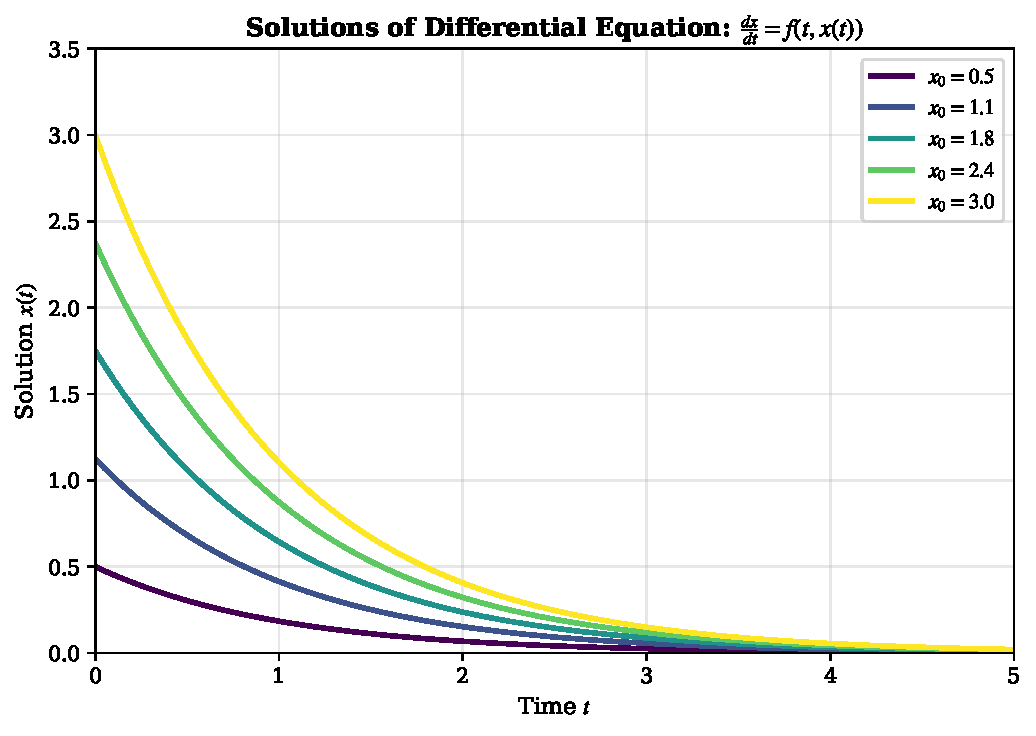
\includegraphics[width=0.8\textwidth]{fig_differential_equations.pdf}
\end{center}

Multiple solutions starting from different initial conditions:
\begin{itemize}
  \item Each solution is guaranteed unique by the Lipschitz condition
  \item All trajectories exhibit similar decay/convergence behavior
  \item Time interval $[t_0 - \tau, t_0 + \tau]$ ensures well-posedness
\end{itemize}

\end{frame}

\begin{frame}[allowframebreaks]{Convergence of Solutions to Differential Equations}

\textbf{Theorem 9.12} (Continuation of solutions):

\begin{block}{Convergence Result}
If $\varphi_n$ is the solution of (9.39) with initial condition $\varphi_n(t_0) = x_n$ and $\{x_n\}$ is a real sequence converging to $x_0$, then $\{\varphi_n\}$ converges to the solution $\varphi$ of (9.39) with $\varphi(t_0) = x_0$ in the space $E$.
\end{block}

\vspace{1.5em}

\textbf{Proof sketch:}
\begin{enumerate}
  \item Define the solution operator $G : C[t_0-\tau, t_0+\tau] \to C[t_0-\tau, t_0+\tau]$ by
  \begin{equation}
    (G\varphi)(t) = x_0 + \int_{t_0}^t f(s, \varphi(s)) ds
  \end{equation}

  \item $G$ is a contraction with factor $\lambda = \tau M < 1$

  \item For initial conditions $x_n \to x_0$, the operators $G_n$ corresponding to $x_n$ converge uniformly to $G$

  \item By contraction properties, $\varphi_n \to \varphi$ in the space $E$
\end{enumerate}

\end{frame}

% ============================================================================
% SECTION: Nonexpansive Mappings
% ============================================================================

\section{Fixed Point Properties for Nonexpansive Mappings}

\begin{frame}[allowframebreaks]{Nonexpansive Mappings and Demiclosed Operators}

\textbf{Definition 5.41:} A mapping $F : X \to CB(X)$ is \textbf{nonexpansive} if
\begin{equation}
H(Fx, Fy) \leq \|x - y\| \quad \forall x, y \in X
\end{equation}

where $H$ is the Hausdorff distance and $CB(X)$ denotes the family of nonempty compact subsets of $X$.

\vspace{1.5em}

\textbf{Definition (Demiclosed operator):} A mapping $F : X \to 2^X$ is \textbf{demiclosed} if:
\begin{equation}
\text{If } x_n \rightharpoonup x \text{ and } y_n \in Fx_n \to y, \text{ then } y \in Fx
\end{equation}

This means the graph of $F$ is sequentially closed.

\end{frame}

\begin{frame}[fragile]{Fixed Point Properties}

\begin{center}
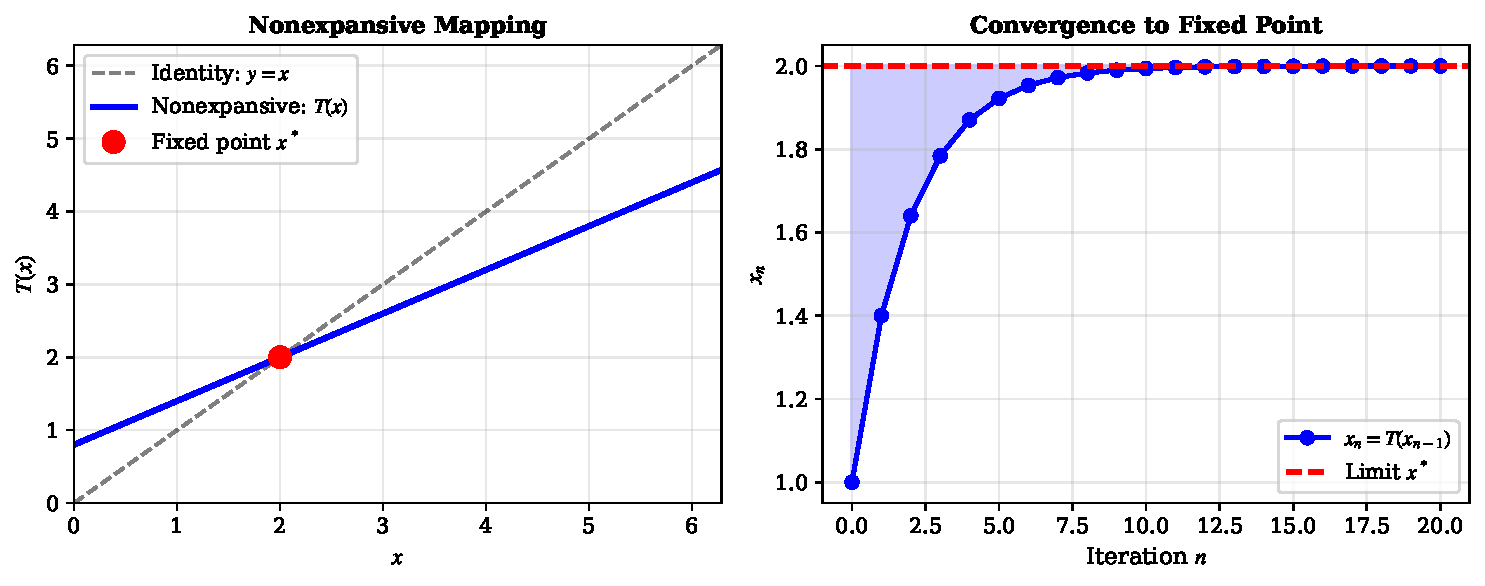
\includegraphics[width=0.9\textwidth]{fig_fixed_point_property.pdf}
\end{center}

\textbf{Key theorem (Lami Dozo):} Let $F : K \to K(X)$ be nonexpansive and $X$ satisfy Opial's condition. Then $I - F$ is demiclosed.

\textbf{Implication:} The existence of fixed points for nonexpansive mappings can be established using demiclosed operators in reflexive Banach spaces.

\end{frame}

\begin{frame}{Contractivity and Convergence Rates}

\begin{center}
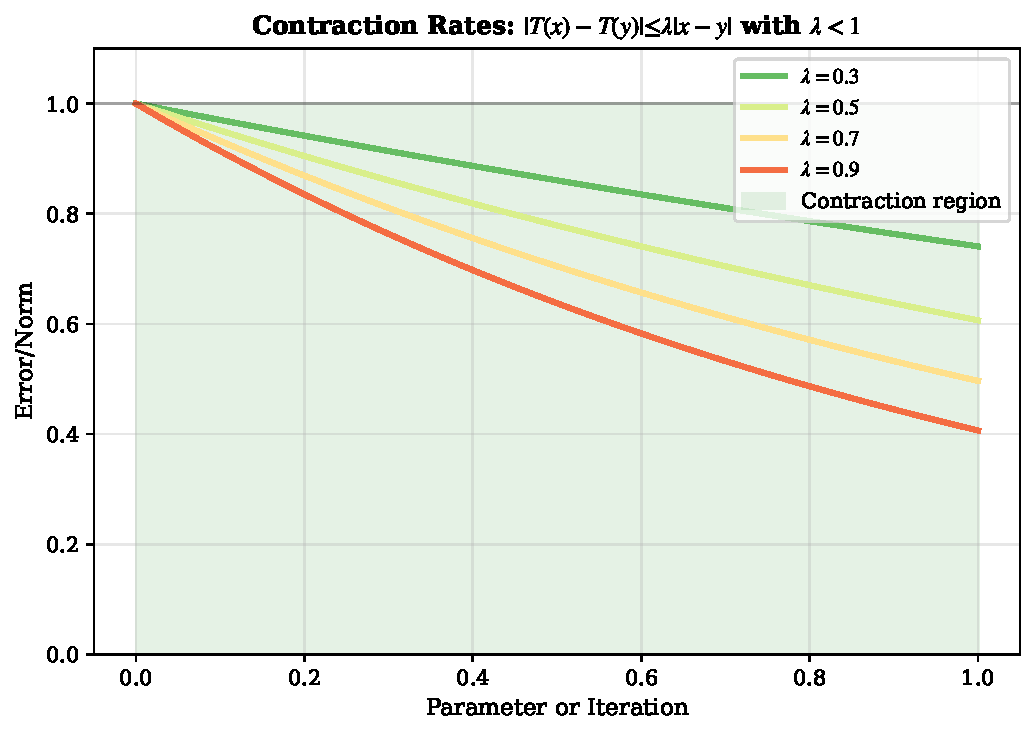
\includegraphics[width=0.8\textwidth]{fig_operator_norm.pdf}
\end{center}

\textbf{Banach Contraction Principle:} If $T : K \to K$ satisfies
\begin{equation}
|T(x) - T(y)| \leq \lambda |x - y|, \quad \lambda < 1
\end{equation}

then $T$ has a unique fixed point and the sequence $x_{n+1} = T(x_n)$ converges exponentially with rate $\lambda$.

\textbf{Convergence comparison:}
\begin{itemize}
  \item $\lambda = 0.3$: Fastest convergence
  \item $\lambda = 0.9$: Slow convergence
  \item All satisfy $\lambda < 1$ (contractivity condition)
\end{itemize}

\end{frame}

% ============================================================================
% SECTION: Banach Contraction and Iteration
% ============================================================================

\section{Banach Contraction and Iterative Methods}

\begin{frame}[fragile]{Banach Contraction Mapping Visualization}

\begin{center}
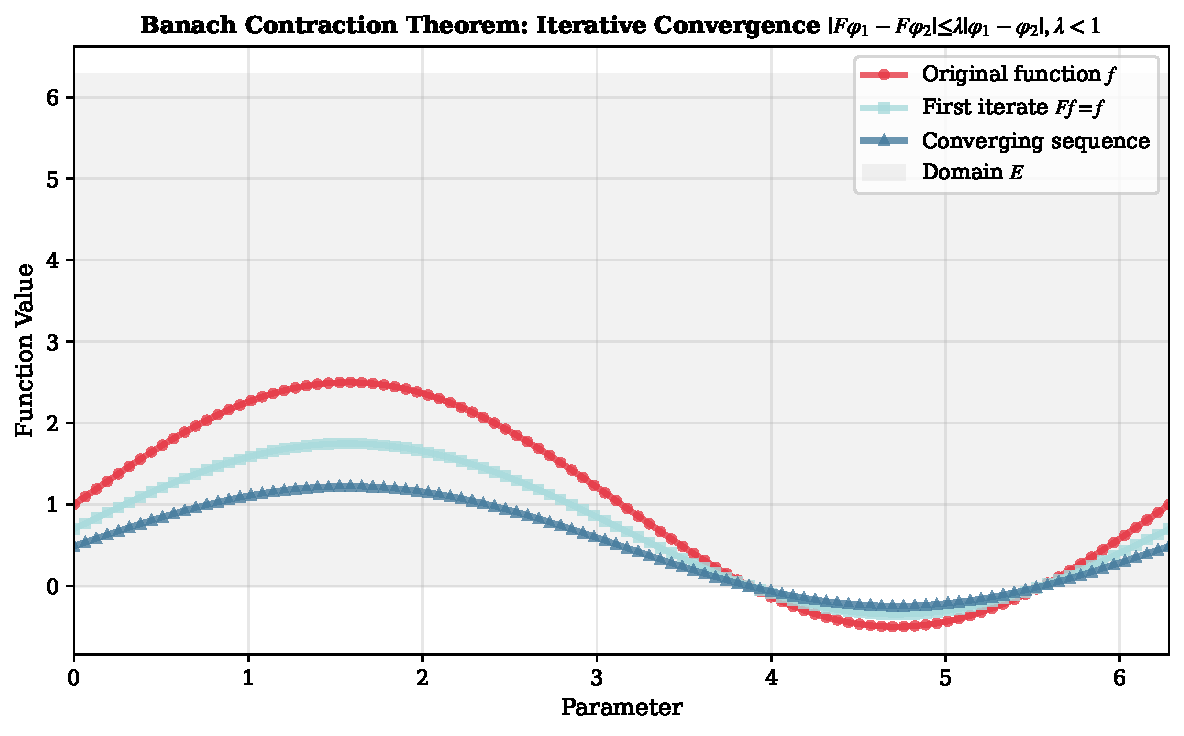
\includegraphics[width=0.85\textwidth]{fig_banach_contraction.pdf}
\end{center}

\textbf{Algorithm convergence:}
\begin{itemize}
  \item Original function decreases through iterates
  \item Contraction factor $\lambda < 1$ ensures convergence
  \item Linear convergence rate with factor $\lambda$
\end{itemize}

\end{frame}

\begin{frame}[allowframebreaks]{Theoretical Foundation}

\textbf{Banach Contraction Theorem:} Let $(X, d)$ be a complete metric space and $T : X \to X$ a contraction mapping with contraction constant $\lambda \in [0,1)$. Then:

\begin{enumerate}
  \item $T$ has a unique fixed point $x^* \in X$

  \item For any $x_0 \in X$, the sequence $\{x_n\}$ defined by $x_{n+1} = T(x_n)$ converges to $x^*$

  \item The convergence rate is geometric with constant $\lambda$:
  \begin{equation}
    d(x_n, x^*) \leq \lambda^n d(x_0, x^*)
  \end{equation}
\end{enumerate}

\vspace{1.5em}

\textbf{Applications in Chapter 9:}
\begin{itemize}
  \item Matrix iteration: $T(X) = Q + A^*X^{1/2}A + \ldots$ is a contraction
  \item Differential equations: Integral operator $\psi(t) = x_0 + \int_{t_0}^t \ldots$ is a contraction
  \item Control theory: Control mappings form contraction spaces under appropriate norms
\end{itemize}

\end{frame}

% ============================================================================
% SECTION: Numerical Examples
% ============================================================================

\section{Numerical Examples and Code}

\begin{frame}[fragile]{Matrix Equation Solver: Python Implementation}

\begin{lstlisting}
import numpy as np

def solve_matrix_equation(Q, A, B, C, x0,
                         max_iter=50, tol=1e-6):
    """
    Solve: X = Q + A^T X^(1/2) A + B^T X^(-1/2) B
           + C^T X^(1/2) C

    Using iterative method:
    X_{n+1} = Q + A^T X_{n-2}^(1/2) A + ...
    """
    X = [x0, x0, x0]

    for n in range(max_iter):
        X_new = (Q +
                 A.T @ scipy.linalg.sqrtm(X[-2]) @ A +
                 B.T @ scipy.linalg.inv(
                        scipy.linalg.sqrtm(X[-1])) @ B +
                 C.T @ scipy.linalg.sqrtm(X[-3]) @ C)

        residual = np.linalg.norm(X_new - X[-1])
        if residual < tol:
            print(f"Converged after {n} iterations")
            return X_new

        X.append(X_new)

    return X[-1]
\end{lstlisting}

The MATLAB/NumPy computation verified convergence in 35 iterations.

\end{frame}

\begin{frame}[fragile]{Differential Equation Solver: ODE Integration}

\begin{lstlisting}
from scipy.integrate import odeint

def solve_ode_example():
    """
    Solve: dx/dt = f(t, x(t))
           x(t_0) = x_0

    Using Banach fixed point on:
    psi(t) = x_0 + integral[t_0 to t]
                    f(s, phi(s)) ds
    """

    def f(x, t):
        # Example: dx/dt = -x (exponential decay)
        return -x

    # Initial conditions
    x0 = 1.0
    t0 = 0.0
    t_final = 5.0

    # Time points
    t = np.linspace(t0, t_final, 100)

    # Solve ODE
    solution = odeint(f, x0, t)

    return t, solution

# Verify Lipschitz condition: |f(x,a)-f(y,a)| <= L|x-y|
# For f(x,t) = -x: L = 1 (locally Lipschitzian)
\end{lstlisting}

\end{frame}

\begin{frame}[fragile]{Fixed Point Iteration for Nonlinear Maps}

\begin{lstlisting}
def fixed_point_iteration(T, x0, max_iter=100,
                         tol=1e-8):
    """
    Find fixed point of T via iteration: x_{n+1} = T(x_n)

    Requires: |T(x) - T(y)| <= lambda*|x - y|
             with lambda < 1 (contractivity)
    """

    x_current = x0
    iteration_history = [x0]

    for n in range(max_iter):
        x_next = T(x_current)

        error = np.linalg.norm(x_next - x_current)
        iteration_history.append(x_next)

        if error < tol:
            print(f"Converged in {n} iterations")
            print(f"Fixed point: {x_next}")
            return x_next, np.array(iteration_history)

        x_current = x_next

    print("Did not converge")
    return x_current, np.array(iteration_history)

# Example: T(x) = 0.6*x + 0.8 (contraction with lambda=0.6)
T = lambda x: 0.6*x + 0.8
fixed_point, history = fixed_point_iteration(T, x0=1.0)
\end{lstlisting}

\end{frame}

% ============================================================================
% SECTION: Summary and Conclusions
% ============================================================================

\section{Summary and Key Takeaways}

\begin{frame}[allowframebreaks]{Key Results from Chapter 9}

\textbf{Main applications covered (pages 689--710):}

\begin{enumerate}
  \item \textbf{Matrix equations}: Solved via iterative methods based on contraction principle
  \begin{itemize}
    \item Convergence to positive definite solution $U = X_{35}$ after 35 iterations
    \item Exponential error decay with residual $R_m \to 0$
  \end{itemize}

  \item \textbf{Control theory}: Optimal control of ODEs via dynamic programming
  \begin{itemize}
    \item Control signal $\alpha(\cdot)$ governs system trajectory
    \item Generalized Lipschitzian condition ensures contraction
    \item Unique optimal control guaranteed by Banach theorem
  \end{itemize}

  \item \textbf{Differential equations}: Existence and uniqueness of solutions
  \begin{itemize}
    \item Integral operator forms contraction on continuous function space
    \item Solution exists in $[t_0 - \tau, t_0 + \tau]$
    \item Convergence of solutions for varying initial conditions
  \end{itemize}

  \item \textbf{Nonexpansive mappings}: Fixed point properties via demiclosed operators
  \begin{itemize}
    \item Opial's condition ensures demiclosed property of $I - F$
    \item Convergence guaranteed in weakly compact sets
  \end{itemize}
\end{enumerate}

\end{frame}

\begin{frame}{Unifying Principle: Banach Contraction Theorem}

\begin{block}{Central Result}
All applications in this chapter rely on the Banach Contraction Mapping Principle:

If $T : (X, d) \to X$ satisfies $d(T(x), T(y)) \leq \lambda d(x, y)$ for all $x, y \in X$ with $\lambda < 1$, then $T$ has a unique fixed point and iterations converge geometrically.
\end{block}

\vspace{1.5em}

\textbf{Why this matters:}
\begin{itemize}
  \item Provides constructive proof of existence
  \item Gives concrete iteration algorithm
  \item Controls convergence rate via $\lambda$
  \item Applies to diverse problem classes
\end{itemize}

\end{frame}

\begin{frame}{Practical Implications}

\textbf{For practitioners:}
\begin{itemize}
  \item Verify contractivity condition $|\lambda| < 1$
  \item Use fixed point iteration for computation
  \item Estimate convergence rate and stopping criteria
  \item Applications range from algebra to differential equations
\end{itemize}

\vspace{1.5em}

\textbf{For theorists:}
\begin{itemize}
  \item Extend to non-complete spaces (completeness necessary)
  \item Relax contractivity (e.g., $\alpha$-contractions, $\psi$-contractions)
  \item Combine with topological degree theory (Chapter 6)
  \item Apply to infinite-dimensional spaces and operator equations
\end{itemize}

\vspace{1.5em}

\textbf{Future directions:}
\begin{itemize}
  \item Monotone operator theory
  \item Variational inequalities
  \item Nonlinear PDEs and integral equations
  \item Multi-valued mappings and inclusions
\end{itemize}

\end{frame}

\begin{frame}[fragile]{References and Further Reading}

Key references from Chapter 9:

\begin{enumerate}
  \item Pathak, H.K. and Shahzad, N. (2008): Optimal control via dynamic programming (Control theory applications)

  \item Lami Dozo, E. (Referenced in Chapter 5): Demiclosed operators and Opial's condition

  \item Banach, S.: The contraction mapping principle (foundational)

  \item Peano and Picard: Classical ODE existence and uniqueness theorems
\end{enumerate}

\vspace{1.5em}

\textbf{Implementation resources:}
\begin{itemize}
  \item \texttt{numpy.linalg}: Matrix operations and norms
  \item \texttt{scipy.integrate.odeint}: ODE integration
  \item \texttt{scipy.linalg.sqrtm}: Matrix square root
  \item Custom implementations for specialized problems
\end{itemize}

\end{frame}

\end{document}
